\documentclass{beamer}
\usepackage[english,russian]{babel}
\usepackage[utf8]{inputenc}
% Стиль презентации
\usetheme{Warsaw}
\begin{document}
\title{Автоматическое выделение терминов для тематического моделирования}  
\author{Никитина Мария}
\institute{Московский физико-технический институт

Факультет прикладной математики и информатики

Кафедра интеллектуальных систем

\vskip 0.2in

Консультант: Потапова Полина

Научный руководитель: д.ф.-м.н. Воронцов Константин Вячеславович}
\date{4 мая 2023 года} 
% Создание заглавной страницы
\frame{\titlepage} 

\begin{frame}{Цели исследования}
\begin{itemize}
    \item Создание алгоритма автоматического выделения терминов в коллекции документов.
    \item Сравнение результатов работы вероятностной тематической модели и нейронной сети.
\end{itemize}
\end{frame}

\begin{frame}{Обозначения}
\begin{block}{Вероятности}
$p_{\omega d}$ -- вероятность появления терма $\omega$ в документе $d$

$\phi_{\omega t}$ -- вероятность того, что терм $\omega$ относится к теме $t$

$\theta_{td}$ -- вероятность встречи темы $t$ в документе $d$
\end{block}

\begin{block}{Матрицы}
$P = (p_{\omega d})_{W \times D}$ -- матрица частот термов в документах

$\Phi = (\phi_{\omega t})_{W \times T}$ -- матрица термов тем

$\Theta = (\theta_{td})_{T \times D}$ -- матрица тем документов
\end{block}

\begin{block}{Множества}
$W$, $D$, $T$ -- множества всех термов, документов и тем соответственно
\end{block}
\end{frame}

\begin{frame}{Постановка задачи}
\begin{block}{Задача}
Найти разложение $P = \Phi\Theta$ с помощью максимизации логарифма правдоподобия:

$\sum\limits_{d \in D}\sum\limits_{w \in d}n_{\omega d}\ln\sum\limits_{t \in T}\phi_{\omega t}\theta_{td} \to \max\limits_{\Phi, \Theta}$
\end{block}

\begin{block}{Проблема}
В общем случае решение задачи не единственно, поэтому задача считается некорретно поставленной по Адамару.
\end{block}

\begin{block}{Решение}
Добавление регуляризаторов $R_i(\Phi, \Theta)$ с неотрицательными коэффициентами регуляризации $\tau_i$, $i = 1, ..., k$. Новая задача:

$\sum\limits_{d \in D}\sum\limits_{w \in d}n_{\omega d}\ln\sum\limits_{t \in T}\phi_{\omega t}\theta_{td} + R(\Phi, \Theta) \to \max\limits_{\Phi, \Theta}$ 

$R(\Phi, \Theta) = \sum\limits_{i = 1}^k\tau_i R_i(\Phi, \Theta)$
\end{block}
\end{frame}

\begin{frame}{Регуляризаторы}
\begin{block}{Декоррелирование}
$R(\Phi) = -\frac{\tau}{2}\sum\limits_{t \in T}\sum\limits_{s \in T\backslash t}\sum\limits_{\omega \in W}\phi_{\omega t}\phi_{\omega s}$

Отвечает за степень различия между темами
\end{block}

\begin{block}{Сглаживание-разреживание}
$R(\Phi, \Theta) = \sum\limits_{t \in T}\sum\limits_{\omega \in W}\beta_{\omega t}\ln\phi_{\omega t} + \sum\limits_{d \in D}\sum\limits_{t \in T}\alpha_{td}\ln\theta_{td}$

Сглаживание применяется для фоновых тем, куда собираются слова, не имеющие определённой темы. Разреживание -- для предметных тем.
\end{block}
\end{frame}

\begin{frame}{Критерии качества}
\begin{block}

$TP$ -- истинно-положительное решение

$FP$ -- ложноположительное решение

$FN$ -- ложноотрицательное решение
\end{block}

\begin{block}{Precision -- точность}
$\text{Precision} = \frac{TP}{TP + FP}$
\end{block}

\begin{block}{Recall -- полнота}
$\text{Recall} = \frac{TP}{TP + FN}$
\end{block}

\begin{block}{F1}
$\text{F1} = 2 \cdot \frac{\text{Precision} \cdot \text{Recall}}{\text{Precision} + \text{Recall}}$

Среднее гармоническое между Precision и Recall
\end{block}
\end{frame}

\begin{frame}{Датасет}
\begin{block}{ACL RD-TEC}
\small Для обучения модели используется открытый датасет ACL RD-TEC, в котором собраны статьи на английском языке с 1965 по 2006 год из области компьютерной лингвистики. Для проведения эксперимента из него удаляются документы, содержащие менее 20 терминов. В результате получается датасет из 9,095 статей.
\end{block}

\begin{figure}
   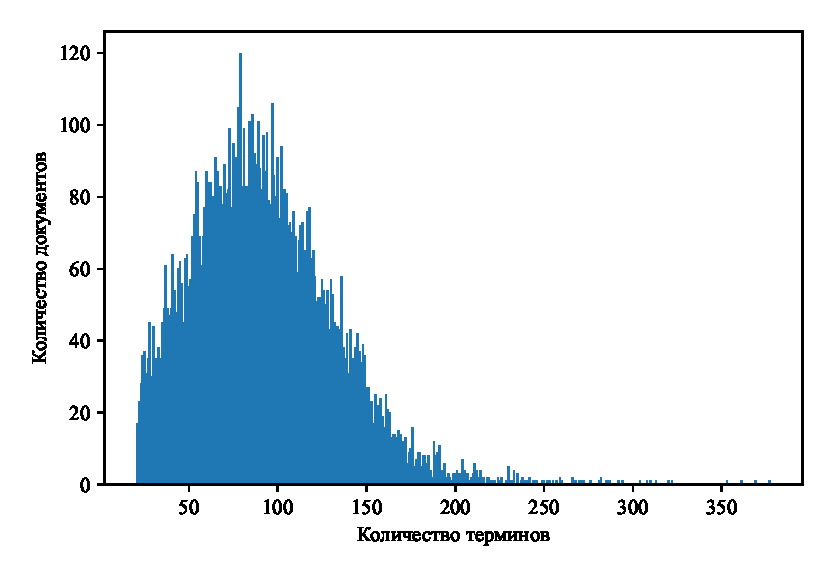
\includegraphics[width=0.475\textwidth]{Pictures/Statistics.eps}
   \hfill
   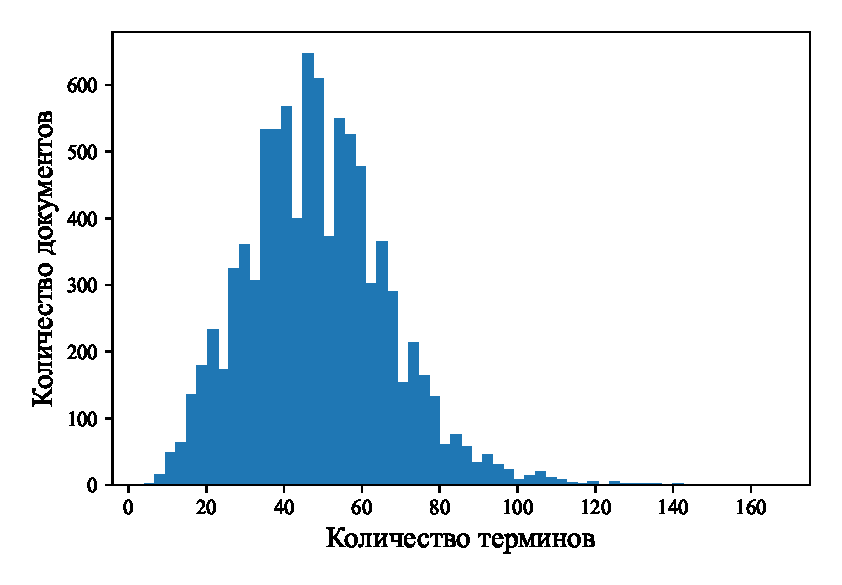
\includegraphics[width=0.475\textwidth]{Pictures/Statistics_1.eps}
\end{figure}
\end{frame}

\begin{frame}{Обработка текста}
Из текста удаляются заголовки, литература, числа и стоп-слова. Также документы подвергаются стеммингу -- отбрасыванию окончаний слов.

\begin{block}{До}
The paper also presents an evaluation of the system 
which shows that the system successfully retrieves the identification numbers of approximately 80\% of the parts.
\end{block}

\begin{block}{После}
paper present evalu system show system success retriev identif number approxim part
\end{block}
\end{frame}

\begin{frame}{Алгоритм}
Текст обрабатывается двумя алгоритмами: TopMine и вероятностной моделью с помощью библиотеки BigARTM. После чего берётся пересечение результатов работы.

\begin{block}{TopMine}
Оценка частота вхождения термина в документ. Позволяет оценивать частоту термина, неслучайность последовательности слов в термине.
\end{block}

\begin{block}{ARTM}
Решение задачи стохастического матричного разложения с добавлением дополнительных регуляризаций.
\end{block}
\end{frame}

\begin{frame}{Работа BigARTM}
\begin{block}{Фоновая тема}
'lie', 'apl', 'ion', 'tire', 'aud', 'tha', 'thc', 'arc', 'rel', 'lit'
\end{block}

\begin{block}{Предметные темы}
['candidate', 'model', 'distance', 'method', 'measure', 'probability', 'language', 'approach', 'based', 'performance']

['document', 'term', 'relevant', 'topic', 'approach', 'information', 'relevance', 'result', 'query', 'number']
\end{block}
\end{frame}

\begin{frame}{BERT}
Для сравнения используется предобученная модель BERT из библиотеки transformers.
\begin{table}[]
\caption{Пример данных для обучения}
\begin{tabular}{|l|l|l|}
\hline
sentence\_id & words          & labels \\ \hline
1            & customer       & O      \\ \hline
1            & service        & O      \\ \hline
1            & allowing       & O      \\ \hline
1            & users          & O      \\ \hline
1            & retrieve       & O      \\ \hline
1            & identification & B      \\ \hline
1            & numbers        & O      \\ \hline
\end{tabular}
\end{table}
Пометка 'O' --- слово не является термином.

Пометка 'B' --- слово является термином.
\end{frame}

\begin{frame}{Результаты}
\begin{table}[ht]
    \caption{Результаты работы алгоритмов}
    \label{table:TopMine}
    \centering\medskip
    \begin{tabular}{|l|l|l|l|}
    \hline
        & Precision & Recall & F1 \\ \hline
        TopMine & 0.063 & 0.946 & 0.117 \\ \hline
        Вероятностная модель & 0.426 & 0.281 & 0.338 \\ \hline
        BERT & 0.636 & 0.732 & 0.681 \\
        \hline
    \end{tabular}
\end{table}
\begin{block}{Выводы}
Вероятностная модель хорошо работает в сравнении с TopMine, но BERT показывает результат лучше. Однако недостатком нейронной сети является большое потребление оперативной памяти и памяти графического процессора. Также, в отличие от вероятностной модели, она неинтерпретируема.
\end{block}
\end{frame}

\begin{frame}{Дальнейшие задачи}
\begin{enumerate}
    \item Использование датасета ACTER, для которого имеется большое количество результатов применения различных методов. Его минус в том, что он небольшой.
    \item Анализ термов из нескольких слов.
    \item Анализ информации о документе: авторы, год издания, заголовок, литература.
\end{enumerate}
\end{frame}

\begin{frame}{Результаты}
\begin{figure}
   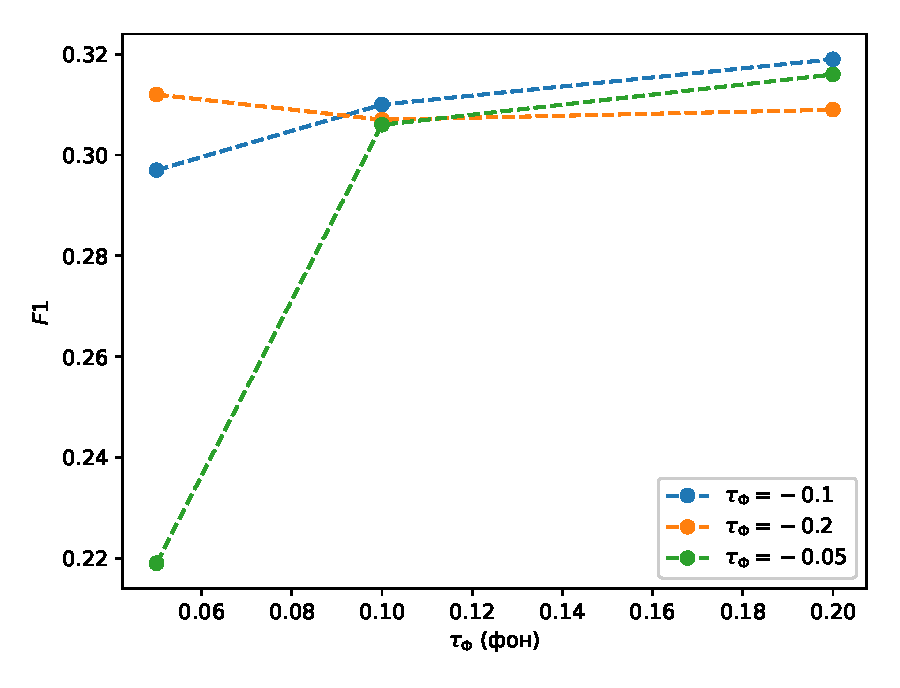
\includegraphics[width=1.0\textwidth]{Pictures/Results.eps}
\end{figure}
\end{frame}

\begin{frame}{Литература}
\begin{thebibliography}{5}
\beamertemplatebookbibitems
\bibitem{A}
\small{\sc Воронцов К.В.}, {\em Вероятностное тематическое моделирование: теория, модели, алгоритмы и проект BigARTM}.
\bibitem{B}
{\sc Ahmed El-Kishky and Yanglei Song and Chi Wang and Clare R. Voss and Jiawei Han}, {\em Scalable topical phrase mining from text corpora}.
\bibitem{C}
{\sc Николай Шаталов}, {\em Методы обучения без учителя для автоматического выделения составных терминов в текстовых коллекциях}.
\bibitem{D}
{\sc Tran,  Hanh Thi Hong and Martinc,  Matej and Caporusso,  Jaya and Doucet,  Antoine and Pollak,  Senja}, {\em The Recent Advances in Automatic Term Extraction: A survey}.
\bibitem{E}
{\sc Behrang Q. Zadeh and Siegfried Handschuh}, {\em The {ACL} {RD}-{TEC}: A Dataset for Benchmarking Terminology Extraction and Classification in Computational Linguistics}.
\end{thebibliography}
\end{frame}
\end{document}